
	This chapter describes the tests made to understand the advantages and problems of the use of the implemented interfaces, also the results from the tests are presented. This chapter makes a effort in justifying the choices made for the tests, such as the test subjects selection.

	The main goal of the tests was to compare the several interfaces developed, to identify important issues to be solved in future works done with this devices, and to understand to which type of tasks might each type of interface adapt better.

	For the tests we have chosen a group of ten male and female subjects who have a broad age range from twenty years old to sixty years old, but most of the group is around their twenties. Nearly all of the subjects use computers every day, in their everyday job, but are not technical users, and have had none or very little contact with the \ac{Wiimote} and no contact with Kinect device, for most of them it was the first time that they even heard about such a interaction device as the Kinect.
	
	The subjects were chosen with these characteristics because we believe that a user with a very little knowledge about the robot and of this type of interfaces might encounter more unexpected difficulties than a user that already knows the iCub limitations or has a very good understanding of how the interface works. This way the main difficulties in controlling the iCub, and most intuitive control methods stand out in a much clearer way.

	The users were invited to come to the Institute for Systems and Robotics - Lisboa, where the iCub robot is kept, to participate in the tests for this thesis. Most of the tests were done during the weekends so that the users could feel comfortable to execute the tests without any distractions, and to comment about their experience.

\section{Tests description}
\label{sec:testsDescription}

	The experience proposed to the user involved a brief presentation about what was the project and what were the tests, a set of tests with different interfaces, and a questionnaire with questions about their experience.
	
	The initial presentation is shown in appendix \ref{appendix:Tests presentation}. The intent with this presentation was to explain what is the iCub robot, what is its objective, why are the tests being done, how do the interfaces that were going to be used worked, and how do the interface devices work. During the tests a presentation slide with detailed information, or with a picture illustrating how the interface worked was shown on a computer screen, as a support to the user test goal. Before each test the user was reminded about how the interface worked, what was the goal of the test, and special details that should be taken into account, such as the fact that the robot did not have any kind of protection about self injury and what were the interface limits.
	
	\begin{table}[htb]
	\begin{center}
		\begin{tabular}{|c|c|c|c|c|}
		\hline
			\backslashbox { Control }{ Device }			& Graphical	& \ac{DPad} 						&	\ac{Wiimote} 	&	Kinect 		\\ \hline
	  	\multicolumn{1}{|c|}{Motor} 						& - 				& - 										& Motor					& Skeleton	\\ \hline
	  	\multicolumn{1}{|c|}{Kinematic} 				& \ac{GUI} 	& \ac{Wiimote} Cursor		& Kinematic 		& Hand 			\\ \hline	  
		\end{tabular}
	\end{center}
	\caption[User tests per control and device]{User tests per control and device.} 
	\label{tab:testsTable}
	\end{table}
	
	Table \ref{tab:testsTable} shows the tests made per device and control type. The control could be made either kinematic or through motor joints independently, and the devices used were a graphical interface, a directional pad, the \ac{Wiimote}, and the Kinect. For the Graphical interface and for the \ac{DPad} only the kinematic control was used, because after a simple try out test with an experienced user the task with the motor control was considered too complex to be done by a novice user, due to having to control each motor independently one at a time.
	
	All the tests were made using the same setup scenery. This scenery is presented in figure \ref{fig:icubTestScenary}, where it is possible to notice that all the objects are suspended from the ceiling, and reachable by the iCub robot right hand. The objects are numbered from one to five to be easily identified by the user. In the task where an obstacle should be present the object number two, shown in figure \ref{fig:icubTestScenary}, was substituted by a blank A4 paper sheet. The user could stand wherever it was more comfortable for the interaction, except during the \ac{GUI} test, because there was the need to use a specific computer, that was next to the iCub robot. The test observer stayed next to the robots emergency shut-down button, and with a extra \ac{Wiimote} in hand that was programmed to position the robot into its initial safe position.
	
	\begin{figure}[htb]
	\centering
	  \subfloat[Front view.]{\label{fig:icubTestSceneryFront}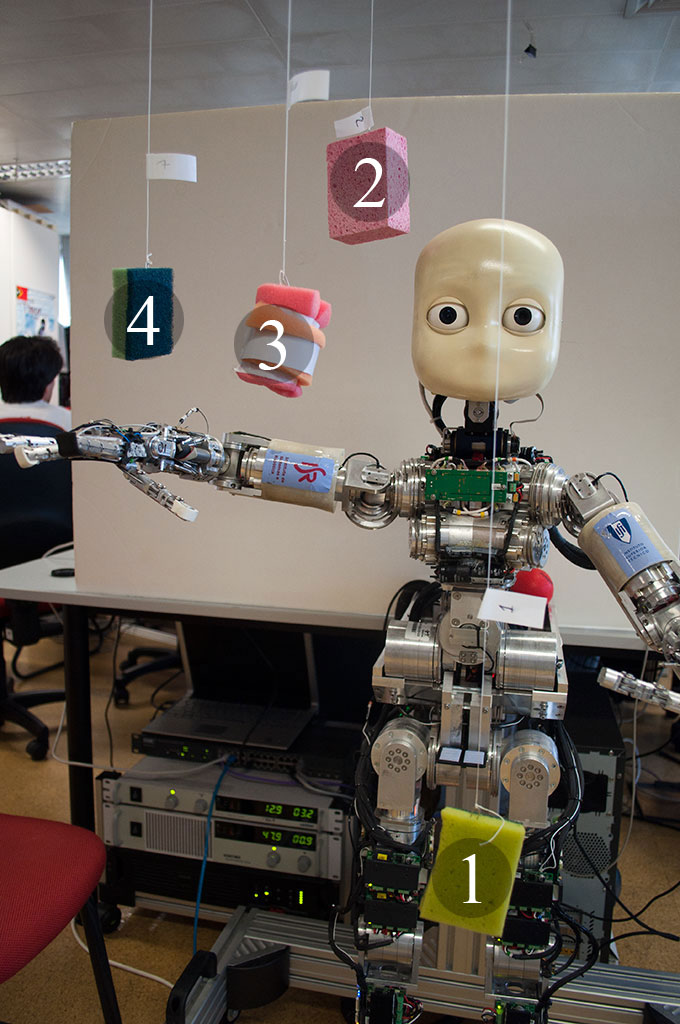
\includegraphics[width=60mm]{testSceneryFront.jpg}}
  \hspace{5mm}
	  \subfloat[Left view.]{\label{fig:icubTestSceneryLeft}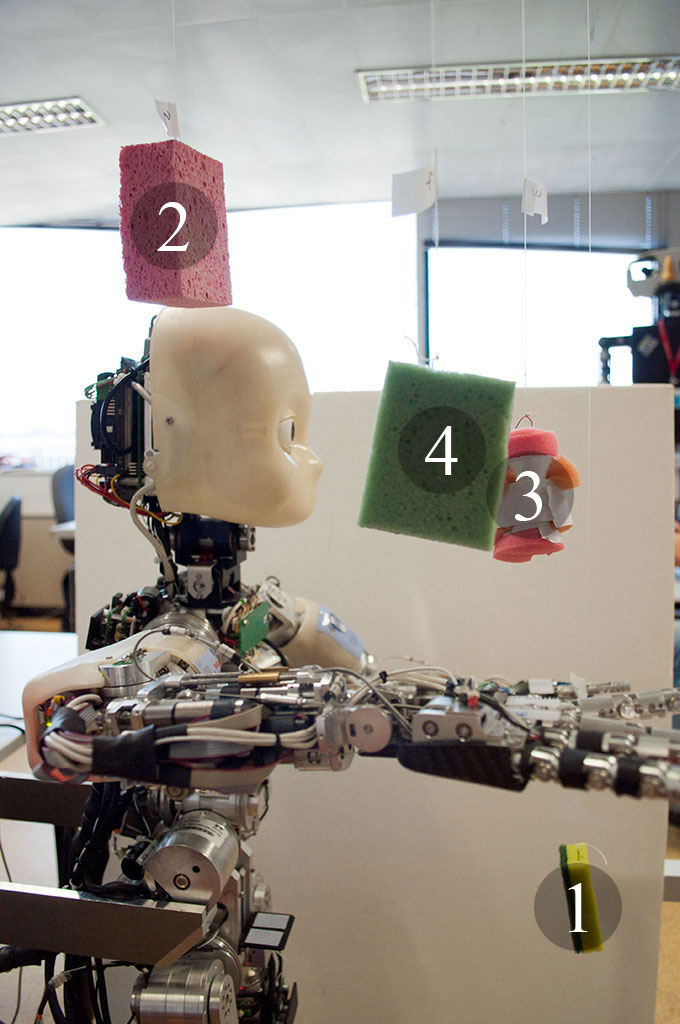
\includegraphics[width=60mm]{testSceneryLeft.jpg}}
	\caption[Interfaces test scenery]{Interfaces test scenery.} 
	\label{fig:icubTestScenary}
	\end{figure}
		
	Each test is divided into five tasks, that are common to all tests. 
	
	\begin{enumerate}
		\item Play with the interface until it is comfortable.
		\item Move hand up and down.
		\item Move hand left and right.
		\item Touch all the objects by the predefined order (1,2,3,4).
		\item Touch some of the objects by the predefined order, with an obstacle (4,1,2).
	\end{enumerate}
	
	The first three tasks were made so that the user could get accustomed with the interface, and to check that the user was able to do basic tasks with the interface, tests would not continue until the user was able to do the second and third tasks in a sufficiently effective way, they are considered basic tasks. During these tasks only the users comments and notes about the interaction were taken. The fourth and fifth tasks are advanced tasks, from this tasks the duration that each task needs to be done is also registered by the program. Before the fourth and fifth were started, the arm would be moved to its initial position making a 90� angle with the side of the robot, and the forearm perpendicular to the arm.
	
	The tasks were made with the intention of testing the user ability to through the interface do a predetermined path with key points, and also how constrains in that path might affect the user experience. The order was chosen so that the user would have to make always a long path and a short path, from object 1 to 2, or from object 4 to 1 is a long path, from object 2 to 3 or 2 to 1 was a short path. Through this we hope to be able to understand what kind of interaction might serve better to what purpose, and how is it possible to make it work better.
	
	Besides these five tasks there were two extra tasks, these tasks were specifically designed for the \ac{Wiimote} kinematic interaction method, and for the Kinect skeleton interaction. With the \ac{Wiimote} kinematic interaction it was asked users to control the orientation of the hand and do simple movements, such as turning the hand upside down and waving. With the Kinect skeleton interaction it was asked to the users to make the iCub robot imitate several poses made by the tests observer. The reason for this tests was that both of these systems were extremely well received by some of the expert users that tried out the interfaces, and it was interesting to see how the non expert users reacted. The tests were extra because they were tasks too simple to be evaluated as the more complex tests.
	
	Before an advanced task took place it was reminded to the user the rules of the task. In the forth task the user should not touch the objects besides the next one in sequence. Although the main focus was to touch all the objects, so if an unintended object was touched a note would be taken but there would be no problem. In the fifth task the user should not touch the obstacle or any of the non intended objects, a non intended object being any other than the next in the supposed sequence. Both of the tasks should be done calmly, control was preferred to speed, and also it was considered more useful not having a shut-down error, such as the robot self-collision than having a task done very quickly.
	
	A test set was composed of five tasks per each interaction method, resulting in sixty tasks to be done. The first task would consume much time because of all the doubts that the user had, the third and second tasks were very quick and none of the users failed. To do each test set a user would need from one hour and a half to two hours, taking into account all the explanations that were given, being that the useful testing time, duration of the advanced tasks four and five for all the devices, took in average forty minutes.

\section{Tests results}

%explain what do the errors mean (shutdown vs restart)
	The tests were evaluated in amount of time and number of errors.
	
	The amount of time was calculated as the total time that it took a user to do the task requested. During the tasks some users stopped to do questions and to think about what should their next action be, to get a better control. The times presented have taken that into account. The times were divided by task and by each object touched.
	
	The number of errors is divided between wrong object touched, reboot, quit, default error, and obstacle touched. A wrong object touched error indicates that the iCub robot touched a non-intended object. A reboot error indicates that a task needed to be restarted due to some problem related with the user interaction. The problem can vary from the robot self collision, to a robot part breaking. A quit error indicates that a user as quit from doing the task. A default error is a unspecified error that occurred at that time from the user interaction. An obstacle touched error indicates that a user touched the obstacle.
	
	A comparison between the average time it takes to conclude an advanced task (tasks 4 and 5) is presented in figure \ref{fig:taskTimeCompare}. The graph shows the average time that it takes a user to finish an advanced task with each one of the control methods. From the graph it is clear that the \ac{GUI} interface is the one that takes the longest and the \ac{Wiimote} cursor (the \ac{DPad} interface) is the fastest control method. The avoid obstacle task with most of the interfaces takes a little less time probably because it was the second time users tried to reach the same objects, and this time there were three objects instead of four. In the case of the Kinect Kinematic (Hand) test there was a big difference between the touch objects test and the avoid obstacle test, this happened because users did larger movements in the second test as a way to deviate from the obstacle, this technique resulted in faster movements from the iCub robot.

	\begin{figure}[htb]
	\begin{center}
	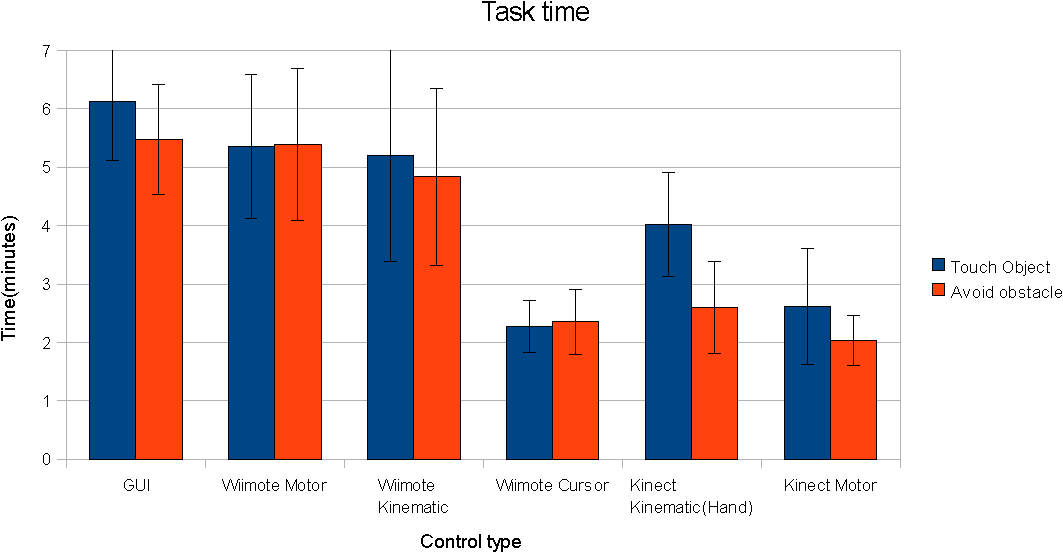
\includegraphics[width=130mm,page=1]{graphsPDF-crop.pdf}
	\end{center}
	\caption[Task time comparison]{Task time comparison.} 
	\label{fig:taskTimeCompare}
	\end{figure}
	
	A comparison between the average amount of errors occurring in the object touch task and the obstacle avoid task in all the interactions is shown in figure \ref{fig:taskErrorCompare}. It can be easily understood that the interaction with the less errors is the \ac{Wiimote} cursor, where both tasks have equal average amount of errors occurring. The \ac{GUI} and the \ac{Wiimote} kinematic interaction are the ones where the most errors take place. The \ac{Wiimote} motor and the Kinect motor (Kinect skeleton) interaction have similar amount of errors, although while observing the users reactions to the interface one could understand that the Kinect motor was much more successful, in time, speed of learning and user involvement. The Kinect kinematic (Kinect hand) interaction had the same amount of errors for both tasks, and from what was observed it was clear that, with the exception of the \ac{Wiimote} cursor interaction which is a typical cursor already known by all the users, this was where the control of what the robot was doing was made in a easier form to the user. With the Kinect kinematic interaction users seemed to have a clear sense of what would the robot do next and how to make it react as it was intended.
	
	\begin{figure}[htb]
	\begin{center}
	\includegraphics[width=130mm,page=2]{graphsPDF-crop.pdf}
	\end{center}
	\caption[Task error comparison]{Task error comparison.} 
	\label{fig:taskErrorCompare}
	\end{figure}
	
	In figure \ref{fig:taskTouchObjectsSteps} it is shown the average time of the touch object task to make the robot end-effector (hand) travel from the initial position to the first object, from the first object to the second, the second to the third and the third to the forth. As it was described before a path needed to be followed during the tasks, the path for this task was defined by the numbers of the objects shown in figure \ref{fig:icubTestScenary}. The first two objects were the ones further way from each other and from the hands initial position, so it is natural that this was the most time consuming maneuver, it was a surprise to see that the Kinect motor control was extremely fast in reaching the first object, the reason why the time to reach the second object peaks is not only because a user to reach the second object needed to deviate from other objects in the way, while the path to the first object did not have any objects, but also because there was an unresolved issue on the position  users tend to take to reach object two, this issue is better explained in the \ref{sec:importanIssues} section. In the figure \ref{fig:taskErrorCompare} it is also clear that the \ac{GUI} interaction is the one that takes more time to reach all the objects except when reaching the fourth object, which was right next to the left of the third object. During the \ac{Wiimote} motor many questions would be made because the control was not very clear, specially while trying to touch the first object, although the intent of the first basic tasks was to avoid this, having a more complex goal than making the robot arm go up, down and to the sides, made the users feel more insecure, although after these doubts were clear the amount of time to reach each object would decrease.
	
		\begin{figure}[htb]
	\centering
	  \subfloat[Touch objects task steps time.] {\label{fig:taskTouchObjectsSteps}\includegraphics[width=120mm,page=4]{graphsPDF-crop.pdf}}
  \vspace{2mm}
	  \subfloat[Avoid obstacle task steps time.] {\label{fig:taskAvoidObstacleSteps}\includegraphics[width=120mm,page=3]{graphsPDF-crop.pdf}}
	  \caption{Tests steps time.}
	  \label{fig:testSteps}
	\end{figure}
	
	The avoid obstacle task consisted in touching on three objects without colliding with an obstacle placed in the middle of the path, as described in section \ref{sec:testsDescription}. In figure \ref{fig:taskAvoidObstacleSteps} is shown the average time to reach each object in the test. The first object was very near the initial position of the hand and could be easily reached, the path that needed to be done to the second and third object were the hardest challenges to solve. The graph \ref{fig:taskAvoidObstacleSteps} is better understood if it is seen with the errors graph \ref{fig:taskAvoidObjectErrors}, because the times achieved with some of the interfaces meant also a high level of errors. Focusing solely in the avoid obstacles time graph it is easy to notice that the Kinect motor interaction was the most successful along with the \ac{Wiimote} cursor interaction. As before these were the interfaces with which the users felt most comfortable. The Kinect motor task actually has a faster time to reach the second object than the first, this happens because when the control starts with this interface the first movements done by user tend to be more to make sure that the robot is actually mimicking the movements correctly than to reach the first object. The \ac{GUI} and the \ac{Wiimote} motor are the slower interactions, but although the \ac{Wiimote} kinematic time to reach the second object seems very good by comparison, in the graph \ref{fig:taskAvoidObjectErrors} it easily noted that there were many errors that accompany this result.
	
	A comparison between each type of error per interaction control type for the touch object task is shown in figure \ref{fig:taskTouchObjectErrors}. In this graph it is clear that the \ac{Wiimote} kinematic control is the less precise control having the higher amount of wrong objects touched, although as it is pointed out in the previous section, the main focus of this task was not to avoid the objects but to follow a path defined by key point objects, but of course wrong object collision avoidance would be considered a plus for good control. The lower error rates are associated with the \ac{Wiimote} cursor interaction and the \ac{Wiimote} motor interaction. The \ac{Wiimote} motor interaction proved to be not so efficient as some of the other interaction control methods, but a better control could be made. The Kinect motor interaction also had a higher level of wrong objects touched, but from the observer perspective it was clear that the user took a riskier control, were higher speed and more difficult movements where made, for example moving the hand through two objects close to each other. Crossing the observer perspective with this results it would be fair to assume that although the control was better with the \ac{Wiimote} cursor and the \ac{Wiimote} motor interaction, the users seemed to be more confident with the Kinect motor interaction. The reboot error happened with two different users, one because the robot self collided, the other because a movement was considered too dangerous by the observer and the emergency shutdown button had to be pressed. The quit error happened because the two older test users gave up after not being able to execute the task, the \ac{Wiimote} kinematic control was not the most successful control type but with this two users, one sixty seven another fifty six years old, it was very hard for them to feel comfortable doing the proposed tasks. The default error is better explained in section \ref{sec:importanIssues}, sometimes it was difficult to detect the user with the Kinect interface, but for most of the users there was no problem.
	
	\begin{figure}[htb]
	\begin{center}
	\includegraphics[width=130mm,page=5]{graphsPDF-crop.pdf}
	\end{center}
	\caption[Error types for the touch object task]{Error types for the touch object task.} 
	\label{fig:taskTouchObjectErrors}
	\end{figure}
	
	To compare the avoid obstacle task errors there is an extra error indicating when a user touched the obstacle, as it can be seen in figure \ref{fig:taskAvoidObjectErrors}, and the main focus of the task was to touch all the object without touching the obstacle. The interaction with less errors was the \ac{Wiimote} cursor control interaction, the only errors occurring in this case were wrong objects touched. The \ac{Wiimote} cursor was also the only interaction where the obstacle was never touched. There were two interaction were user quit, the main reasons were very low confidence in that the task could be completed, and one user after having successive self collisions with the robot it was considered best to skip to the next test. The reboot happened in most cases because the observer was not confident that the user would be able to make a certain movement without either self collision, or moving the robot to an dangerous position where parts could be broken, as it happened with one of the users where one of the iCub robot cable was broken even though the limits set by the iCubInterface should avoid this. The \ac{Wiimote} kinematic control was the one with the higher value of times the obstacle was touched, demonstrating how little precision the users were able to have during this control method. In the touch object task the users during the Kinect motor control opted for doing riskier movements as a way to shorten the time for a specific test and also they wanted to feel how well the robot could be controlled with that system, this was mainly due to the excitement of having a robot humanoid mimicking their movements. Because the \ac{Wiimote} motor control and the \ac{Wiimote} kinematic control appealed to the user for their intuition instead of logic, although the \ac{Wiimote} motor worked better once it was understood as several younger users showed, in this test the lack of precision would increase the difficulty of the task conclusion, so some users facing that they could not conclude the task properly opted by quitting the task and proceeding to the next task.
	
	\begin{figure}[htb]
	\begin{center}
	\includegraphics[width=130mm,page=6]{graphsPDF-crop.pdf}
	\end{center}
	\caption[Error types for the avoid object task]{Error types for the avoid object task.} 
	\label{fig:taskAvoidObjectErrors}
	\end{figure}
	
	Through the notes and execution times taken during the tests it is possible to consider the \ac{GUI} interaction as the less efficient interaction, and the \ac{Wiimote} cursor as the most efficient and with the best control interaction. Nevertheless it can not be overlooked the fact that the users had a better involvement while executing the Kinect motor task, and even with being a never used before interface, which is not the case with the \ac{Wiimote} cursor, it had very good results in terms of efficiency and of user confidence in the interaction.
	
\section{Questionnaire results}

	After the users had finished the tests, a web based questionnaire was given, and they were reminded that the questionnaire should be filled taking into account that the goal was to compare the interfaces, understand the weak points and most important issues to be resolved. The questionnaire can be seen in the appendix \ref{appendix:questionnaire}.
	
	The questionnaire was composed of eighteen questions, the first six were about the user characteristics, such as if the user had ever used the interface devices, age, and profession. The following twelve had directly to do with the interaction experience, most of the questions where either multiple choice questions or ranking questions, there were only two questions were a written response was asked. Because the tests were directed to non technical users, most of the answers available to choose from the questionnaire are written in a subjective form, although in all the questions the first answer was the most negative and the last one was the most positive.
	
	All of the users considered the initial description of the interaction method being evaluated as clear, but as it was already pointed out, there  were questions about the specificity of each interaction as the tasks were being done. The professional occupation of each test user was very different, with only one user, a student, having a technological background. All the users spend time with a computer every day, but only two users had any contact with a \ac{Wiimote} like device and one owned a Wii gaming console, no user had ever interacted with a Kinect device. the users age varied between twenty years old and sixty seven years old, but most of the users were around twenty years old.
	
	The exact results from the questionnaire can be consulte in the appendix \ref{appendix:questionnaireResults} in the form of percentage tables and percentage graphs.
	
	The questionnaire can be divided into two main questions groups, questions about the users difficulty during the interaction experience, and questions ranking the interaction control types. One more question about the extra task done was also asked.
	
	From the questions directed to the users interaction difficulties the \ac{Wiimote} kinematic was the control type where the users felt that the robot responded in the least expected way, and the \ac{Wiimote} cursor where the users felt that the expected reaction was met during the interaction. There was also a high value of correct expectations about the Kinect motor (Kinect skeleton) control.
	
	The \ac{GUI} control was where the users were less preoccupied, about what the reaction of the robot might be, transmitting a good sense of control, probably the fact that only one type of movement could be made at a time, as pointed in section \ref{sec:importanIssues}, contributed to this result, obliging the users to focus on one movement at a time. The Kinect motor control was the one with the highest value of preoccupation from the user, this preoccupation is influenced by the fact that the users did not trust that the interface would replicate their pose in an accurate way. In the \ac{Wiimote} motor control users did not feel either too preoccupied nor too relaxed about the interaction.
	
	When the users were questioned if they felt disoriented, not clear if they were controlling the robot correctly while using the interface, only the \ac{Wiimote} kinematic control stands out as the one with worst results, because much of the control is done based on intuition rather than in a logical form. In contrast the \ac{Wiimote} cursor control and the Kinect motor control were considered very clear, the users always had a good understanding of how they were controlling the robot.
	
	As for precision the \ac{Wiimote} cursor control, the Kinect hand control, and the Kinect skeleton control were the controls that obtained top grade voting, while the \ac{Wiimote} kinematic control was where the grades where lower so less precision was felt by the users. The \ac{GUI} was considered better than the \ac{Wiimote} motor control, but none of them got the higher rating.
	
		\begin{table}[htb]
	\begin{center}
		\begin{tabular}{c|c|c|c|c|c|c|}
		\cline{2-7}
		&  \ac{GUI}	& \ac{Wiimote} 	& \ac{Wiimote} 	& \ac{Wiimote} 	& Kinect 	& Kinect 		\\
		&  					& motor					& kinematic			& cursor				& hand 		& skeleton	\\ \hline
	  	\multicolumn{1}{|c|}{Best for task} 				& 4 & 5 & 6 & 1 & 3 & 2\\ \hline
	  	\multicolumn{1}{|c|}{Preferred by the user} & 3 & 4 & 3 & 2 & 2 & 1\\ \hline	  
		\end{tabular}
	\end{center}
	\caption[Interaction control ranking]{Interaction control ranking.} 
	\label{tab:interactionRanking}
	\end{table}
		
	There were two ranking questions, where users were asked to rank the several interaction systems used, by personal preference and by what they thought to be the best system to do the tasks that were requested, the results of this ranking are shown in table \ref{tab:interactionRanking}. The users voted the \ac{Wiimote} cursor control as the best interaction system to do the tasks requested, and the \ac{Wiimote} kinematic system as the worst interaction control. To understand the user involvement and satisfaction with each system by comparison, the top ranked system was the Kinect skeleton, and the last ranked system was the \ac{Wiimote} motor. The \ac{Wiimote} cursor, the Kinect hand, and the Kinect skeleton control, were the three top ranked system in both questions.
	
	The questionnaire ended with two selection question about the orientation and pose extra tasks, this questions were made to have some evaluation of the very simple tasks requested to the users. The interaction in the \ac{Wiimote} hand orientation task was considered ``good'', and the interaction in the Kinect pose task was considered ``very good'', that are the top two classifications of five possible to choose.

\section{User comments}

	During the users tests, the observer would take notes on user comments, most of the comments were done during the interactions considered harder, as the \ac{GUI}, \ac{Wiimote} motor, and \ac{Wiimote} kinematic interactions, but comments would be made through out all the tests.
	
	The scenery was considered by many users as clear, and did not create any doubts about the tasks requested. Although objects one and two were distinguished by users for being the hardest ones to reach.
	
	During the \ac{GUI} test many users complain about the obligation to move in one axis at a time. The controls were considered straight forward but, the fact that the \verb|x| axis was negative to the front of the robot and positive to the back of the robot made the control confusing. To avoid this confusion one user made a note of the controls direction before starting the tests, the same user suggested that instead of having solely the axis information having also name labels with the words: up; down; right; left; back; front; might make the interface clearer. One of the most repeated complains was related to the fact that a user is not able to stop the control once it has begun, a stop button would suffice to fix this problem.
	
	During the \ac{Wiimote} motor tests the ability to stop a move the robot when the user wants, that is available in all interfaces except the \ac{GUI}, was appreciated and commented by several users. The concept of the interaction was difficult to pass on to most of the users, with the exception of the engineering student, who had a technical background, and after understanding how the joint motors of the iCub were mapped to the \ac{Wiimote} was very comfortable with the interaction. The forearm control was limited to two motors, being simpler than the arm, that has three motors, although a user commented that the forearm was harder to control conveniently.
	
	During the \ac{Wiimote} kinematic tests some users commented that their position relatively to the robot had an influence on how they performed, because this oblige the users to control in a mirrored way. It was also indicated that this was a dificult control form to interpreter, because no spatial notion of the end-effector was present. Users were worried with the movements control due to the robot speed that was higher than in the previous tests, at the same time there was a feeling that the robot had a delay that did not help the control. The orientation that the end-effector (hand) took was also commented on, because the users did not have nay control over that.
	
	During the \ac{Wiimote} cursor tests users felt that this was the most comfortable method, but that the delay experienced was a issue, that influenced the users performance.
	
	During the Kinect kinematic hand test comments were many times to the fact that the mapping of movements to the robot could be made in other way, because it became not so clear. The user detection problems were also an issue due, because it obliged users to re do the calibration process again. The fact that control could be set on and off with the \ac{Wiimote} button, was considered very useful.
	
	During the Kinect skeleton motor test users commented on the dificulty in controlling the robot around object two. The interface system was considered very simple, but it was uncomfortable not to have complete notion of what speed the robot could achieve with an unintended faster movement. Also the position that the user picked initially most of the times didn't allow to see the robot completely in a clear way, specially in the obstacle task.
	
	As overall comments users pointed out the usefulness of a graphical interface and some form of feedback to some of the interactions, although it was explained that this was intentionally kept out. Also a module for detection of self collision that would stop the robot from damaging it self, would have helped to make the users less worried during the interaction.
	
	After the tests and in a informal way, even with all the issues that can be resolved, users considered that the interaction systems developed, could be useful for a different number of tasks, were fun, practical.

\section{Important issues}
\label{sec:importanIssues}

	There are several issues that were noted, and repeatedly commented on that should be better explained.

	The \ac{GUI} control was already developed by a developer of the iCub community, but it might be good to suggest a few alterations, the most noted was the fact that only a movement in a axis could be made at a time, by directly changing the sliders. Allowing for more movements can bring a higher risk but also a faster control from the user.
	
	The Kinect device is a very new device, so some issues remain to be upgraded, although in most cases it worked without any difficulties. One issue was that with one specific user, that was using not too tight clothes as indicate by the manufacture that it should, was very hard to detect, and re-calibration had to be re-done several times.
	
	When using the Kinect skeleton motor control, reaching object two became difficulty because this was at the limit of one of the motors. By our implementation, when a user tries to reach a certain angle in a motor that is beyond the limit, the motor stops immediately. This option was taken as a precaution against unexpected movements that might be requested to the motor from the interfaces.
	
	Although it was preferred not to have any form of feedback that would facilitate users in their tasks, it seemed clear that having a graphical, sound, or any other type of feedback would affect the way users do the tasks not only depending in the interface they were using but also on the type of feedback they would be able to get. Because the objective was to compare simple interfaces and how people would interact with a humanoid robot through these interfaces only, it was preferred to leave the feedback interfaces created during the development phase out of the user testing, since they could influence the user performance.
	
	During the kinematic controls users were surprised to see that the hand would take arbitrary orientations, the kinematic chain used to control the robot, iKin, was the one resposible for this behavior. With the iKin when a new position is given for the robot to reach, a new pose for the robot is computed, in that pose it is considered two elements, the position to reach and a orientation to define. The orientation could have been defined in a strict way, although after testing this system it was understood that it would limit the reaching ability of the robot, and many times the orientation would oblige the robot to do unexpected movements, so the orientation setting was ignored and only the position is defined.

	With a more specific goal for the interface any of this issues can be resolved to adequate in a better form for the problem, so this are considered important issues, but not critical errors in our systems.

\section{Concluding remarks}

	In this chapter the evaluation tests and its results were presented.
	
	There were a number of different options taken that influenced the results of the tests, two of those options that have had a heavy weight on the results were: the absence of feedback from the interaction systems, other than the robot response, this would allow to evaluate the interface device itself and not depend on the support interface; the test subjects that were chosen with very little technical abilities, hoping that this would make stand out the determinant characteristics in the interaction.
	
	The tests where divided into five tasks from which the amount of time spent doing the task was annotated and also the errors that occurred during the task. Each of the tests was done for each of the control methods, \ac{GUI}, \ac{Wiimote} motor, \ac{Wiimote} kinematic, \ac{Wiimote} cursor, Kinect kinematic hand, and Kinect motor skeleton.
	
	The interaction system with which the users obtained better results was the \ac{Wiimote} cursor. This system was the one users could related the best because the control of avatars and interfaces through \acp{DPad} and key cursors are relatively common in the day to day use of technology. The \ac{GUI} also represents a very common daily used interface, although due to the way it is organize it did not have a good result, users expect most of the times it to be easier to use, and also simpler than three slide bars. The \ac{Wiimote} interaction systems where the gyroscope was used, kinematic and motor systems, were the ones where users found it most difficult to grasp the concept, although in some particular cases it was a very successful system, mostly when used by users with some experience of the device. The Kinect interaction systems, were the most appreciated, and also the ones considered the biggest novelty. Considering that for many of the users it was the first time that such a system was even seen, that the time of learning needed was very small, and the results which were very satisfactory for a system with no support interface, the Kinect was the interface where users felt more envolved.
	
	The tests also allowed us to get to know important issues of the interactions, some that should be enhanced by adding features, others that should be fixed for a better interaction.
